\documentclass[a4paper, 12pt]{article}
\usepackage[left=17mm, top=17mm, right=17mm, bottom=0mm, headsep=1em]{geometry} % лист а4, 12 кегль, тип документа - статья
\usepackage[utf8]{inputenc}  % кодировка вводимого текста
\usepackage[english, russian]{babel}  % подключение словарей с переносами англ и рус яз
\usepackage{amssymb, latexsym, amsmath, mathtext, bm, gensymb, amssymb}  % пакеты для работы с мат символами
\usepackage{indentfirst}  %  каждый абзац с красной строки
\setlength{\parindent}{4ex}
\linespread{0.4} % межстрочный интервал
 
\usepackage{graphicx}
\graphicspath{ {./images/} }

\usepackage{bm}
\usepackage{enumitem}
\usepackage[T2A]{fontenc}

\usepackage{fancyhdr}

\newcommand{\RNum}[1]{\uppercase\expandafter{\romannumeral #1\relax}}

\makeatletter
\AddEnumerateCounter{\asbuk}{\russian@alph}{щ}
\makeatother

\pagestyle{fancy}
\fancyhf{}
\rhead{Саженов Константин Станиславович}
\lhead{Группа М8О-108Б-19}
\chead{Вариант 22}
% \rfoot{Page \thepage}
\setlength{\headheight}{28pt}
% \set

\begin{document}
\section*{Задание \RNum{2}} 
\paragraph{Текст задания} Используя алгоритм Терри, определить замкнутый маршрут, проходящий ровно по два раза
(по одному в каждом направлении) через каждое ребро графа.

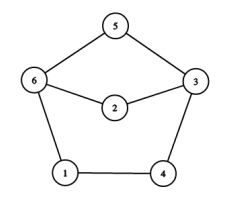
\includegraphics{2_task}

\paragraph{Решение}
$$ 1 \rightarrow 4 \rightarrow 3 \rightarrow 5 \rightarrow 6 \rightarrow 2 \rightarrow 3 \rightarrow 2 \rightarrow 6 \rightarrow 1 \rightarrow 6 \rightarrow 5 \rightarrow 3 \rightarrow 4 \rightarrow 1$$
\end{document}